\chapter{KAJIAN PUSTAKA}
\label{chap:chap2_kajian_pustaka}

\section*{}
Demi mendukung penelitian ini, dibutuhkan beberapa teori penunjang sebagai bahan acuan dan referensi. Berikut adalah paparan teori dasar meliputi komponen desain permainan, \textit{machine learning}, dan penjelasan permainan genre RPG (\textit{Role-Playing Game}).
\vspace{1ex}

\section{Kajian penelitian terkait}
\label{sec:sec2_kajian}
\vspace{1ex}

Beberapa penelitan sebelumnya yang berkaitan dengan penelitian ini dan mendukung penelitian ini antara lain:

\begin{enumerate}
	\item Paper dengan judul ``\textit{Measuring Level of Difficulty in Game Using Challenging Rate (CR) on 2D Real Time Strategy Line Defense Game}" yang ditulis oleh Christyowidiasmoro dan rekan-rekan tahun 2015. Meneliti tentang formula \textit{Challenging Rate} (CR) adalah formula yang menggunakan elemen dasar dalam permainan RTS (\textit{Real Time Strategy}) sebagai parameternya. Dalam tulisan ini dibuat sebuah \textit{prototipe} permainan dengan tingkat kesulitan yang diajukan untuk mencoba kemampuan formula \textit{Challenging Rate} untuk mengukur nilai tingkat kesulitan.

	\item Paper dengan judul ``\textit{A game engine to make games as multi-agent systems}" yang ditulis oleh Carlos Marín-Lora dan rekan-rekan tahun 2019. Pada tulisan ini meneliti tentang pengembangan \textit{game engine} yang berfokus pada multi-agen. Di mana pada setiap aktor atau agen-agen memiliki sejumlah properti dan aturan kebiasaan untuk berinteraksi dengan lingkungan dalam permainan. Tujuan dari engine tersebut adalah memenuhi kebutuhan dasar dari sistem multi agent dengan merubah karakteristik dari system tanpa adanya pengaruh terhadap potensi karakter.

	\item Paper dengan judul ``\textit{Procedurally Generating Game Level with Specified Difficulty}" yang ditulis oleh Zong-Han Wu dan rekan-rekan tahun 2018. Penelitian ini mencakup ranah pembuatan konten dalam sebuah permainan secara prosedural, hal tersebut bertujuan agar para pemain memperoleh pengalaman yang berbeda dalam bermmain. Pada paper ini yang paling banyak di ulas adalah permainan PAC-MAN, dengan labirin yang dapat berubah secara procedural.
	
	\item Paper dengan judul ``\textit{Generating an Attribute Space for analyzing Balance in Single Unit RTS Game Combat}" yang ditulis oleh Shaun Bangay dan Owen Makin tahun 2014. Fokus pada tulisan ini adalah tentang pencapaian keseimbangan dalam permainan \textit{Real Time Strategy} (RTS), dengan dibuatnya sebuah framework yang dinamakan dengan \textit{attribute space}. Pendekatan ini dievaluasi dan direpresentasikan untuk pertarungan \textit{single unit} atau satu lawan satu pada permainan RTS. Melalui proses tersebut kemudian dibuatlah model prediksi terhadap simulasi pertarungan tersebut, dengan menggunakan attribut atau data statistik pada permainan tersebut seperti halnya \textit{speed}, \textit{range}, \textit{health} dan \textit{damage}.
\end{enumerate}

\section{Desain Permainan RPG dan Komponennya}
\label{sec:sec2_gdd}
\vspace{1ex}

Desain permainan adalah proses menciptakan konten dan aturan permainan. Desain permainan yang baik adalah proses menciptakan tujuan agar seorang pemain merasa termotivasi untuk mencapainya dan aturan yang dibuat dapat diikuti oleh seorang pemain saat membuat keputusan untuk mengejar tujuan-tujuan tersebut \citep{Brathwaite2009}. Berikut adalah sebagian elemen dari desain permainan yang akan digunakan pada permainan dengan genre RPG pada penelitian ini.
\vspace{1ex}

\begin{subs}
	\subsection{Penempatan Peluang pada Permainan}
	\label{sec:sub_sec2_kesempatan}
	\vspace{1ex}
	
	Sebagian besar permainan setidaknya mengandung beberapa faktor acak. Misalnya, banyak permainan kartu melibatkan proses acak. Adanya variabel \textit{damage} dipertarungan pada sebagian besar permainan dengan genre RPG. Permainan seperti \textit{Rock-Paper-Scissors} memiliki pola yang tampak acak, meskipun terlihat tanpa mekanisme acak. Pada bagian ini akan banyak membahas mengenai aspek acak pada permainan dan bagaimana \textit{developer} akan menggunakannya.
	\vspace{1ex}
	
	Pada dasarnya permainan yang memasukan unsur keberuntungan dapat dimainkan dan dimenangkan oleh khalayak luas. Bila dicari alasan penggunaannya, hasilnya sangatlah banyak. Pada akhirnya harus diakui bahwa hal-hal tersebut adalah keputusan dari desainer permaninan untuk menciptakan dinamika yang dikehendakinya. Berikut adalah contoh-contoh penerapan penempatan peluang pada permainan yang biasanya diterapkan.
	\vspace{1ex}
	
	\begin{enumerate}[label=\textbf{\alph*).}]
	
		\item \textbf{Menunda atau Mencegah Penyelesaian Masalah}
		\setlength{\parindent}{0.8cm}
	
		Untuk permainan yang memiliki sedikit cara penyelesaian saat dipecahkan oleh komputer dan terutama manusia. Maka sesuatu harus dilakukan untuk menjaga permainan agar tetap \textit{fresh} dan menyenangkan. Di tambahkanlah elemen acak untuk mencapai tujuan tersebut. Hal tersebut bertujuan agak pemain tidak terlalu menguasai permainan, karena saat pemain membuat keputusan yang sama persis dapat memberi hasil yang berbeda. Hal tersebut tentunya juga berpengaruh pada tingkat rasa bosan pemain dalam memainkan sebuah permainan, jika pola yang sama terus muncul.
		\vspace{1ex}
	
		\item \textbf{Membuat Permainan Lebih Kompetitif}
	
		Elemen acak yang sesekali memungkinkan pemain yang kurang berpengalaman untuk menang atau setidaknya menawarkan keuntungan yang membuat permainan ini bertahan lebih lama dengan menggunakan dua cara. Pertama adalah selalu ada peluang kemenangan bagi setiap pemain. Kemudian yang kedua adalah efek dari kekalahan berkurang ketika seorang pemain bisa menyalahkan nasib buruknya sendiri atas kekalahannya. Hal tersebut tentunya juga dapat memunculkan rasa tidak terima akan sebuah kekalahan dan dimulainya permainan baru lagi.
		\vspace{1ex}
		
		\item \textbf{Meningkatkan Keberagaman}
	
		Permainan tanpa elemen acak selalu dimulai dengan cara yang sama dan pola-pola tertentu seperti langkah awal pada permainan Catur. Akibatnya, pemain dapat memiliki pengalaman yang sama dari satu pertandingan ke pertandingan yang lain, dan para pemain dapat mejatuhkan pilihannya untuk selalu memakai strategi yang sama.
		\vspace{1ex}
	
		\item \textbf{Menciptakan Momen Dramatis}
	
		Ketika seorang pemain dengan hati-hati menyusun strategi dan kemudian harus bergantung pada lemparan dadu atau apa pun yang bersifat acak untuk melihat apakah rencana tersebut berhasil, momen tersebut bisa menjadi sangat menegangkan. \textit{Role-Playing Games} (RPG), \textit{Real-Time Strategy} (RTS) dan banyak \textit{board game} yang mengandalkan kondisi ini saat bermain. Akankah \textit{healing spell} (mantra penyembuhan) yang digunakan akan sampai ke rekan bermainmu yang terluka sebelum monster menyerang? Apakah AI akan memberi pemain dua monster untuk bertempur ataukah hanya satu?
		\vspace{1ex}
	
		\item \textbf{Meningkatkan Pengambilan Keputusan}
	
		Inti dari sebagian besar permainan adalah keputusan yang dibuat para pemain. Dalam permainan strategi, pemain memiliki informasi lengkap dan tahu hasil pasti dari setiap gerakan yang mereka lakukan. Karena semua variabel diketahui, beberapa keputusan menjadi tidak terlalu menarik, jika ada kesempatan untuk membunuh ratu lawan pada permainan catur secara cuma-cuma tanpa ada yang perlu dikorbankan, hal tersebut bukan merupakan keputusan yang menarik karena adanya jawaban ``benar" yang jelas. Ketika elemen acak ada dalam permainan, tidak ada lagi strategi yang selalu benar. Beberapa gerakan mungkin memiliki peluang kegagalan yang tinggi tetapi juga potensi hasil yang besar, hal tersebut menjadikannya sebuah pilihan berisiko, gerakan lainnya mungkin aman tetapi menghasilkan sedikit keuntungan. Hal tersebut menjadikan pemain akan melakukan analisis gerakan dengan cara yang berbeda berikut risiko dan keutungan yang akan didapat, kemudian tidak lupa mempertimbangkan posisi pemain tersebut dalam permainan atau langkah selanjutnya.
		\vspace{1ex}
		
	\end{enumerate}
	
	\subsection{Elemen Keterampilan Strategi}
	\label{sec:sub_sec2_strategi}
	\vspace{1ex}
	
	Strategi adalah salah satu kekuatan yang dapat dilakukan oleh para pemain. Karena hal tersebutlah yang membuat para pemain tetap bermain. Pemain bermain \textit{game} dan menikmati setiap prosesnya karena mereka berusaha untuk menguasai pola dalamnya \citep{Koster2013}. Saat pola berhasil dikuasai, maka selanjutnya pemain akan terus bersenang-senang. Mereka juga membentuk strategi berdasarkan pemahaman mereka tentang dinamika permainan. Penguasaan, pengembangan strategi, hal tersebut terjadi bukan karena ketidak sengajaan. 
	\vspace{1ex}
	
	Hal ini adalah tujuan dari desainer permainan atas penggunaan mekanika untuk menciptakan strategi dan taktik dalam permainan yang mereka buat \cite{Brathwaite2009}. Berikut beberapa poin penting pada penelitian ini yang mengacu tentang pentingnya Elemen Keterampilan Strategi.
	\vspace{1ex}

	\begin{enumerate}[label=\textbf{\alph*).}]
		
		\item \textbf{Peran dari Keterampilan pada Permainan}
		\setlength{\parindent}{0.8cm}
	
		Permainan yang bagus dibangun dari serangkaian keputusan menarik, membangun unit untuk menyerang atau bertahan, mencari tahu apa yang harus dilakukan oleh unit tersebut selanjutnya, apa saja kelemahannya dan lain sebagainya. Keberhasilan keputusan tersebut juga didasari oleh reaksi dari mental atau fisik pemain, karena hal tersebut adalah ukuran keterampilan dari seorang pemain.
		\vspace{1ex}
	
		Permainan yang bagus menyebabkan pemain sering melatih kemampuannya dan memberi \textit{reward} atau bonus dengan pola timbal balik yang jelas. Kemudian sepanjang permainan pemain bertanya-tanya tentang apa yang harus dilakukan selanjutnya. Masuklah mereka ke dalam istilah yang disebut dengan ``lingkaran sihir" sebuah \textit{video game}, melalui monitor atau TV sebagai medianya terseraplah mereke ke dalam dunia game. Efek tersebut sama seperti ketika menonton film atau membaca buku yang sangat menarik, tetapi permainan yang baik memiliki daya tarik yang lebih kuat karena terjadi interaksi antara pemain dan keputusan yang dibuat yang terkonversi menjadi sebuah pengalaman.
		\vspace{1ex}
		
		Ketika pemain terus-menerus membuat keputusan, secara tidak sadar mereka telah memasuki kondisi yang oleh psikolog dan peneliti terkenal Mihaly Csikszentmihalyi disebut ``\textit{flow}". Hal tersebut adalah keadaan permainan yang optimal dan merupakan hasil kerja keras dari seorang desainer pemainan. Csikszentmihalyi menulis seluruh buku tentang topik, \textit{Flow: The Psychology of Optimal Experience}. Buku ini tidak terbatas pada permainan saja, tetapi mencakup keadaan semacam ini dari perspektif yang lebih luas.
		\vspace{1ex}
		
		\item \textbf{Strategi dan Taktik}
		
		Secara teknis strategi utama adalah keseluruhan cara untuk mencapai tujuan akhir jangka panjang (misalnya, kemenangan dalam permainan). Strategi utama terdiri dari beberapa strategi pendukung dengan tujuan jangka pendek atau menengah yang harus dilakukan untuk mencapai strategi besar (misalkan dalam peperangan besar, pilihan untuk bertarung dalam pertempuran tertentu adalah sebuah pilihan strategis). Taktik adalah keputusan mikro tingkat terendah yang dibuat ketika menjalankan strategi misalkan pada pergerakan pasukan, apakah akan diperintahkan untuk melakukan serangan udara, kapan pasukan haarus mulai bergerak, dimana posis yang tepat untuk menempatkannya, kapan mulai menembak dan lain-lain adalah contoh keputusan taktis yang dibuat selama pertempuran militer. Secara informal pemain dalam permainan membuat keputusan strategis ketika membuat rencana jangka panjang (panjangnya strategi tersebut bersifat relatif terhadap panjangnya permainan), dan keputusan taktis ketika pemain ingin mencapai tujuan jangka pendek.
		\vspace{1ex}
		
		Pengorbanan mejadikan pengambilan keputusan atau pembuatan taktik menjadi lebih menarik. Keputusan yang diambil secara cepat atau \textit{twitch mechanics}, bisa disebut juga dengan ketangkasan memiliki keterbatasan pada taktik. Hal ini menunjukkan bahwa permainan yang lebih fokus pada strategi, umumnya bersifat giliran atau \textit{turn-based} seperti Catur dan \textit{Go}, yang mana lebih terfokus pada keputusan yang melibatkan pengorbanan.
		\vspace{1ex}
		
		\item \textbf{Game Berbasis Keterampilan Sepenuhnya}
		
		Permainan yang fokus pada strategi dan pengorbanan cenderung memiliki setidaknya beberapa elemen peluang. Ketika permainan-permainan ini murni berbasis keterampilan, seperti \textit{Tic-Tac-Toe} atau sebagian besar \textit{video game} petualangan, mereka dapat diselesaikan, dan keputusan-keputusan yang tadinya bervariasi kemudian menjadi keputusan-keputusan yang jelas. Misalkan dalam membuat keputusan pada akhirnya hanya ada satu gerakan atau pilihan benar.
		\vspace{1ex}
		
		Sebagian besar game yang sepenuhnya berupa keterampilan adalah game aksi berbasis fisik. Mungkin hal inilah sebabnya, tidak seperti pada pengorbanan yang bukan tentang mendapatkan jawaban yang benar atau terbaik melainkan mendapatkannya dengan cepat. Waktu reaksi atau tindakan manusia dapat terus meningkat dari waktu ke waktu selamanya, terutama pada permainan dimana manusia saling berlawanan satu dengan yang lain atau \textit{multiplayer}.
		\vspace{1ex}
	\end{enumerate}

	\subsection{Menemukan Keseimbangan}
	\label{sec:sub_sec2_keseimbangan}
	\vspace{1ex}
	
	Beberapa permainan sangat terlihat jelas bahwa semua membutuhkan keterampilan. Hal ini sangat bervariasi dari yang sederhana (\textit{Tic-Tac-Toe}) menuju yang lebih kompleks (Catur dan \textit{Go}). Ada juga perbedaan antara keterampilan berbasis strategis (seperti pada kebanyakan permainan berbasis strategi dan giliran) dan kemampuan pengambilan keputusan secara cepat atau \textit{twitch} (biasa ditemukan dalam permainan berbasis keterampilan dan olahraga) atau bisa disebut juga dengan ketangkasan. Permainan ini bisa menjadi sangat menyenangkan karena terdapat keputusan berarti yang dibuat oleh pemain, baik itu keputusan yang dibuat dengan cepat (\textit{twitch}) dan keputusan yang dibuat berdasarkan strategi \citep{Brathwaite2009}.
	\vspace{1ex}
	
	Banyak permaian yang menggabungkan kedua basis di atas. \textit{Settlers of Catan} memiliki banyak elemen \textit{gameplay} berbasis keterampilan, termasuk perdagangan, pembangunan, dan manajemen sumber daya. Namun permainan tersebut juga memiliki dadu, setumpuk kartu yang dikocok secara acak, dan pengaturan papan yang disusun dengan acak. \textit{Backgammon} dan \textit{Poker} keduanya memiliki elemen keterampilan dan keberuntungan yang kuat. Bayangkan sebuah permainan \textit{Backgammon} tanpa dadu, atau \textit{Poker} tanpa kemampuan untuk bertaruh atau menggertak lawan, dan menjadi jelas bahwa beberapa permainan mampu menjadi lebih baik dengan adanya campuran keterampilan dan peluang. Jika salah satunya dihapus maka permainan tersebut tidak akan menjadi menarik.
	\vspace{1ex}
	
	Bagaimana seorang desainer permainan memasukkan campuran keterampilan dan peluang yang benar dalam sebuah permaian? Kapan saat yang tepat untuk mengarahkan permainan ke arah itu? Jawabannya adalah kembali kepada siapakah pemainnya?
	\vspace{1ex}
	
	Hal tersebut adalah pertanyaan penting, seringkali pertanyaan pertama yang diajukan seorang desainer. Ketika merancang permainan untuk anak berusia enam tahun hasil yang diperoleh akan sangat berbeda jika dibandingkan dengan merancang permainan yang diperuntukkan bagi mahasiswa. Pemain yang berbeda memiliki tingkat toleransi yang berbeda untuk setiap peluang dan keterampilannya. Permainan yang mungkin menjadi sangat populer bagi para gadis muda bisa jadi menjadi membosankan bagi orang dewasa, karena sebagai orang tua yang telah memainkan sejumlah permainan anak-anak dan dapat mengujinya. Beberapa contoh target pemain seperti anak-anak, pemain permainan kompetitif, permainan sosial, pemain profesional dan keluarga. Dalam penelitian ini akan difokuskan dengan permainan kompetitif, karena fokus utamanya adalah \textit{fun games}.
	\vspace{1ex}
	
	Pemain permainan kompetitif cenderung lebih menyukai permainan dengan lebih banyak elemen keterampilan. Hal ini memberi mereka kesempatan untuk bermain satu lawan satu dengan pemain lain, mencocokan setiap pemikiran menjadi sebuah strategi, refleks melawan refleks, strategi melawan strategi. Hal terakhir yang diinginkan oleh pemain yang benar-benar kompetitif adalah proses acak seperti halnya dengan penggelindingan dadu yang merusak permainan yang dieksekusi dengan sempurna dan terampil.
	\vspace{1ex}
	
	Mengapa desainer menambah keberuntungan pada permainan berbasis keterampilan? Banyak alasan yang membuat hal-hal tidak dapat diprediksi, meningkatkan kemampuan pemain dengan memainkan permainan itu lagi, dan memungkinkan pemain dengan keterampilan yang sedikit berbeda untuk tetap dapat bersaing. Jika pemain yang lebih baik selalu menang, maka satu-satunya pertarungan yang menarik adalah antara dua pemain dengan kemampaun yang sama rata.
\end{subs}
\vspace{1ex}

\section{Machine Learning}
\label{sec:sec2_ML}
\vspace{1ex}

\textit{Machine Learning} (ML) adalah studi ilmiah tentang algoritma dan model statistik yang digunakan oleh komputer untuk melakukan tugas tertentu secara efektif tanpa menggunakan instruksi secara eksplisit, dengan mengandalkan pola dan inferensi sebagai gantinya. \textit{Machine learning} juga dilihat sebagai bagian dari kecerdasan buatan. Algoritma dari \textit{machine learning} membangun model matematika berdasarkan data sampel, yang dikenal sebagai ``data training" dalam membuat prediksi atau keputusan tanpa diprogram secara eksplisit untuk melakukan tugasnya \citep{Koza1996}.
\vspace{1ex}

Algoritma \textit{machine learning} dapat digunakan pada berbagai aplikasi, seperti penyaringan email, dan visi komputer, yang mana tidak mungkin untuk mengembangkan algoritma instruksi khusus untuk melakukan tugas dengan sendirinya. \textit{Machine learning} terkait erat dengan komputasi statistik yang berfokus pada pembuatan prediksi dengan menggunakan komputer. Studi tentang optimasi matematika memberikan metode, teori dan domain aplikasi ke bidang \textit{machine learning}. Penambangan data atau \textit{data mining} adalah bidang studi yang termasuk ke dalam cakupan \textit{machine learning}, dan berfokus pada analisis dan eksplorasi data melalui pembelajaran yang mampu berjalan secara otomatis \citep{Friedman1997}.
\vspace{1ex}

Pada penelitian ini akan digunakan beberapa algoritma \textit{machine learning} untuk menyelesaikan permasalahan dalam mendesain permainan. Penggunaan algoritma tersebut secara umum adalah membuat data baru yang terstruktur dengan referensi data awal yang disesuaikan dengan kebutuhan untuk mendesain permaian. Berikut algoritma-algoritma tersebut dan penjelasannya secara umum nantinya, di mana natinya akan dipakai dan dijelaskan secara detail pada BAB \ref{chap:chap3_metodologi}.
\vspace{1ex}

\begin{subs}
	\subsection{K-Nearest Neighbor}
	\label{sec:sub_sec2_knn}
	\vspace{1ex}
	
	Di asumsikan terdapat sampel $(x_{i}, \theta_{i})$ yang didistribusikan secara sesuai dengan distribusi $(x, \theta)$ argumen heuristik tertentu yang memungkinkan dalam prosedur pengambilan keputusan. Contohnya saat pengasumsian tentang jarak dari beberapa data, metrik atau koordinat yang sesuai akan diklasifikasi berdasarkan kesamaannya atau setidaknya memiliki kesamaan distribusi pada setiap datanya. Maka dalam klasifikasi sampel $x$, dipertimbangkan berdasarkan $x_{i}$ terdekat yang diasumsikan sebagai kemungkinan terbesar. Sehingga prosedur pengambilan keputusan paling sederhana adalah aturan \textit{nearest neighbor} (NN) dengan mengklasifikasikan $x$ sebagai tetangga terdekat.
	\vspace{1ex}
	
	Di buatlah satu set $n$ pasangan $(x_{1}, \theta_{2}), ..., (x_{n}, \theta_{n})$, yang mana $x_{i}$'s mengambil nilai dalam metrik $X$ yang didefinisikan sebagai metrik $d$, dan $O_{i}$ nilai yang diambil di set $\{1, 2, ..., M\}$ seperti pada persamaan \ref{eq: KNN_all_x_data} dan \ref{eq: KNN_distance}. Setiap $\theta_{i}$ dianggap sebagai indeks dari kategori yang dimiliki oleh data ke-$i$, dan setiap $x_{i}$ adalah hasil dari pengukuran setiap data. Lebih singkatnya pada ``$x_{i}$ bagian dari $\theta_{i}"$ adalah saat data ke-$i$ yang menjadi dasar pengukuran $x_{i}$ yang telah diamati dan diukur, termasuk juga pada kategori $\theta_{i}$.
	\vspace{1ex}
	
	Di lakukan beberapa penambahan pasangan baru $(x,$ $\theta)$, yang mana pengukuran $x$ yang akan dilakukan, dan digunakan hasilnya digunakan untuk memperkirakan $\theta$ dengan memanfaatkan hasil pengukuran atau klasifikasi sebelumnya. Pada persamaan \ref{eq: KNN_all_x_data} dinyatakan bahwa seluruh data $x$ atau $x_{n}$ yang akan diguanakan untuk mecari nilai $\theta$.
	
	\begin{equation}\label{eq: KNN_all_x_data}
	x'_{n}\ \epsilon\ x_{1}, x_{2},\ ...,\ x_{n}
	\end{equation}
	
	\noindent Akan termasuk ke dalam \textit{nearest neighbor} terhadap $x$ jika dilanjutkan dengan persammaan berikut.
	
	\begin{equation}\label{eq: KNN_distance}
	min\ d(x_{i}, x) = d(x'_{n}, x),\ \ \ i = 1, 2,\ ...,\ n
	\end{equation}
	
	Aturan \textit{nearest neighbor} menentukan, apakah $x$ termasuk dalam kategori $\theta'_{n}$ dari tetangga terdekatnya $x'_{n}$ seperti pada persamaan \ref{eq: KNN_distance} di mana metrik $d$ adalah \textit{distance} atau jarak. Kesalahan dibuat jika $\theta'_{n} \neq \theta$. Perhatikan bahwa aturan \textit{nearest neighbor} hanya menggunakan klasifikasi berdasarkan tetangga terdekat saja. Sedangkan $n - 1$ yang merupakan sisa hasil klasifikasi $\theta_{i}$ akan diabaikan \citep{Cover1967}. Dengan demikian, metode klasifikasi berbasis $k-$NN dapat dengan mudah diterapkan dalam banyak tugas klasifikasi. Secara umum, sebagian besar varian $k-$NN menentukan label kelas dari sampel data dengan menggunakan satu parameter $k$ yang merupakan jarak dari keseluruhan data yang di anggap sebagai \textit{neighbour} dan juga keputusan di ambil dengan mempertimbangkan jarak data secara mayoritas. Tetapi keputusan klasifikasi tersebut dapat dengan mudah dipengaruhi oleh sensitivitas $k$ itu sendiri dan juga dapat memperburuk sensitivitasnya, sehingga sangat menurunkan kinerja klasifikasi dari $k-$NN terutama dalam kasus ukuran sampel yang kecil.
	
	\begin{enumerate}[label=\textbf{\alph*).}]
		
		\item \textbf{Klasifikasi}
		\setlength{\parindent}{0.8cm}
		
		Dalam mendemonstrasikan analisis $k-$\textit{nearest neighbor}, dipertimbangkan juga proses klasifikasi objek baru (koordinat data) diantara sejumlah contoh yang diketahui. Hal ini ditunjukkan pada Gambar \ref{fig:k-nn_plus_minus}, yang menggambarkan representasi dari data atau \textit{instance} dengan tanda plus dan minus dan titik dengan lingkaran merah. Dan permasalahan yg harus diselesaikan adalah memperkirakan (klasifikasi) hasil dari titik tersebut berdasarkan sejumlah tetangga terdekat atau \textit{nearest neighbor} yang dipilih. Dengan kata lain, apakah titik tersebut dapat diklasifikasikan sebagai tanda plus atau minus.
		
		\begin{figure} [!h] \centering
			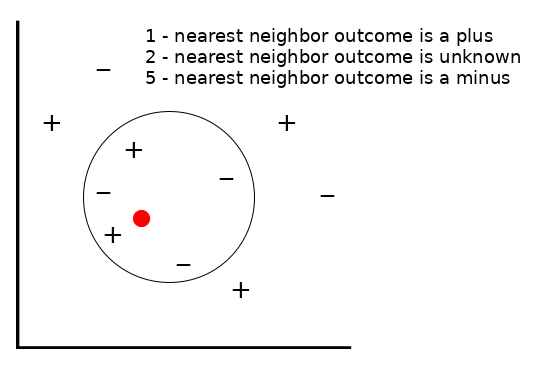
\includegraphics[scale=0.45]{img/k-nn_plus_minus.png}
			\caption{Klasifikasi dengan $k-$NN.}
			\label{fig:k-nn_plus_minus}
		\end{figure}
		
		Kemudian dipertimbangkannya hasil $k-$NN berdasarkan tetangga terdekat pertama (1-\textit{nearest neighbor}). Jelas bahwa dalam hal ini $k-$NN akan memprediksi hasil dari titik atau representsi data dengan nilai tambah (karena titik terdekat adalah tanda plus). Dilanjutkan dengan penambahan jumlah tetangga terdekat menjadi 2 (2-\textit{nearest neighbor}). Kali ini $k-$NN tidak akan dapat mengklasifikasikan hasil dari titik dari data yang dicari, karena titik terdekat keduanya adalah minus, sehingga tanda plus dan minus mencapai jarak yang sama. Untuk langkah selanjutnya, ditambahkan lagi jumlah tetangga terdekat menjadi 5 (5-\textit{nearest neighbor}). Hal ini akan menentukan daerah tetangga terdekat, yang ditunjukkan oleh lingkaran yang seperti pada Gambar \ref{fig:k-nn_plus_minus}. Karena ada 2 tanda plus dan 3 tanda minus. Pada lingkaran tersebut $k-$NN akan memberikan tanda minus pada hasil dari titik koordinat yang dicari.
		
		\item \textbf{Regresi}
		
		Pada bagian ini akan digeneralisasi konsep $k-$\textit{nearest neighbor} untuk menyelesaikan permasalahan regresi. Permasalahan regresi sangat berkaitan dengan prediksi hasil dari variabel dependen berdasarkan beberapa variabel independen. Di mulai dengan mempertimbangkan skema yang ditunjukkan pada Gambar \ref{fig:k-nn_sinosoid}, di mana satu data \textit{training} atau data sampel (kotak jingga) yang diambil dari hubungan antara variabel independen $x$ dan variabel dependen $y$ (kurva biru). 
		
		\begin{figure} [!h] \centering
			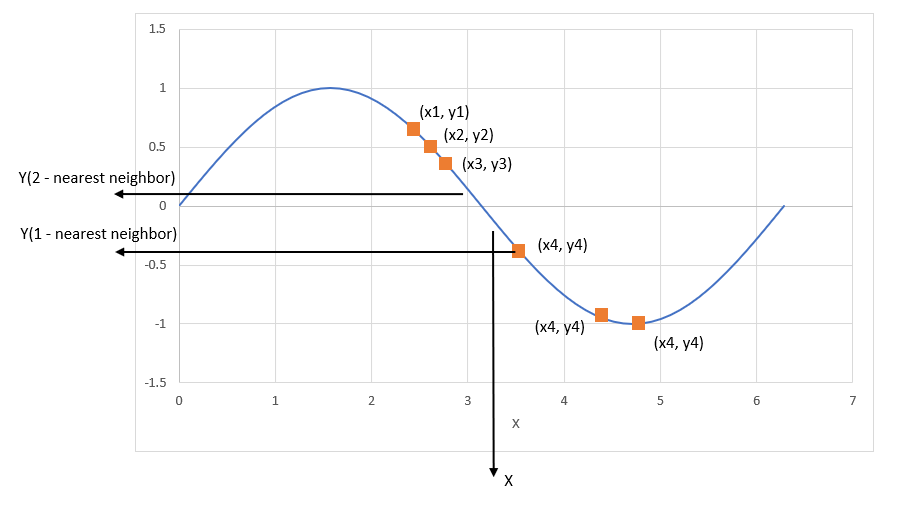
\includegraphics[scale=0.6]{img/k-nn_sinosoid.png}
			\caption{Proses regresi dengan $k-$NN.}
			\label{fig:k-nn_sinosoid}
		\end{figure}
		
		Kemudian ditandai dengan kotak jingga yang dlianjutkan dengan penerapan $k-$\textit{nearest neighbor} untuk memprediksi hasil keluaran yang ditandai dengan $X$. Kemudian direpresentasikan juga dengan kotak jingga. Di mulai dengan mempertimbangkan metode 1-\textit{nearest neighbor} sebagai data sampel. Dalam kasus ini akan dicari data sample (kotak jingga) yang paling dekat dengan titik X. Pada Gambar \ref{fig:k-nn_sinosoid} yang dicari dinyatakan dalam koordinat $(X, Y)$ sedangkan koordinat data yang paling mendekati adalah $(x_{4}, y_{4})$. Maka dapat disimpulkan bahawa tetangga terdekatnya atau \textit{nearest neighbor} adalah $(x_{4}, y_{4})$ untuk 1-\textit{nearest neighbor}.
		\vspace{1ex}
		
		Langkah selanjutnya adalah mencari 2-\textit{nearest neighbor} seperti pada Gambar \ref{fig:k-nn_sinosoid}. Pada kasus ini ditemukan dua titik terdekat dengan X atau 2-\textit{nearest neighbor}, yang kebetulan ditunjukan pada Gambar \ref{fig:k-nn_sinosoid} adalah $y3$ dan $y4$. Maka diambil rata-rata dari masing-masing nilai pada data tersebut yang dinyatkan pada persamaan \ref{eq: KNN_regresi_mean}.
		
		\begin{equation}\label{eq: KNN_regresi_mean}
		\begin{split}
		Y = \frac{y_{3} + y_{4}}{2}
		\end{split}
		\end{equation}
		
		Pada metode $k-$\textit{nearest neighbor} hasil Y dari titik X dianggap sebagai hasil rata-rata dari nilai $k-$\textit{nearest neighbor} dari tetangga terdekatnya.
		\vspace{1ex}
		
		\item \textbf{Cross-Validation}
		
		\textit{Cross-validation} adalah teknik yang dapat digunakan untuk mendapatkan estimasi model parameter yang tidak diketahui. Pembahasan ini bertujuan untuk menerapan teknik dalam memperkirakan nilai $k$. 
		\vspace{1ex}
		
		Gagasan umum dari metode ini adalah untuk membagi sampel data ke dalam sejumlah kelompok atau \textit{cluster} (diambil secara acak, \textit{sub-samples} atau bagian-bagian yang terpisah). Untuk nilai tetap pada $k$, digunakanlah $k-$NN untuk membuat prediksi pada bagian ke $v$ (mislahnya dengan penggunaan bagian $v-1$ sebagai contoh) dan kemudian digunakan untuk evaluasi kesalahan. Metode paling umum untuk analsia kesalahan pada regresi adalah dengan jumlah kuadrat atau \textit{sum of square} dan pada klasifikasi hal tersebut didefinisikan sebagai akurasi atau tingkat kebenaran klasifikasi.
		\vspace{1ex}
		
		Proses ini kemudian diterapkan secara berurutan pada semua bagian atau $v$ yang mungkin. Pada bagian terakhir, kesalahan yang dijumlahkan kemudian dirata-rata untuk menghasilkan model yang stabil (seberapa baik model memprediksi titik koordinat data). Langkah-langkah di atas kemudian diulang untuk berbagai nilai $k$ yang lain, nilai yang mencapai kesalahan terendah atau akurasi klasifikasi tertinggi dijadikan sebagai nilai optimal untuk $k$. 
		\vspace{1ex}
		
		Usaha dalam mencapai nilai optimal inilah yang kemudian disebut dengan \textit{cross-validation}. Perlu diperhatikan bahwa \textit{cross-validation} membutuhkan proses komputasi tinggi dan algoritma harus dibiarkan berjalan untuk beberapa waktu terutama saat ukuran sampel berjumlah besar. Atau nilai $k$ dapat ditentukan sendiri. Ini mungkin tindakan yang wajar jika sudah megetahui apa yang akan diambil sebagai nilai $k$, dari analisis $k-$NN sebelumnya yang mungkin dilakukan pada data yang sama atau pengamatan secara manual.
		
		\item \textbf{Jarak Metrik}
		
		Seperti disebutkan sebelumnya, pada titik data yang dicari, $k-$NN membuat prediksi berdasarkan hasil $k$ dari tetangga terdekat dengan titik itu. Oleh karena itu, untuk membuat prediksi dengan $k-$NN, sangat diperlukan pendefinisian metrik untuk mengukur jarak antara titik koordinat data dan kasus dari data sampel. 
		\vspace{1ex}
		
		Salah satu metode paling populer untuk mengukur jarak ini dikenal dengan istilah \textit{Euclidean}. Langkah-langkah lain diantaranya adalah \textit{Euclidean squared}, \textit{City-block}, dan \textit{Chebyshev} seperti yang ditunjukan pada persamaan \ref{eq:KNN_distance_metrics}.
		\vspace{1ex}
		
		\begin{equation}\label{eq:KNN_distance_metrics}
		\begin{split}
		D(x,\ p) =
		\begin{Bmatrix}
		\sqrt{(x - p)^{2}} & Eclidean\\
		(x - p)^{2} & Eclidean squared\\
		abs(x - p) & Cityblock\\
		Max(|x - p|) & Chebyshev
		\end{Bmatrix}
		\end{split}
		\end{equation}
		
		Di mana pada persamaan \ref{eq:KNN_distance_metrics} variabel $x$ dan $p$ masing-masing adalah titik koordinat data yang dicari dan data sampel. Kemudian yand dimasud dengan D adalah \textit{distance} atau jarak antara data sampel dengan koordinat data yang dicari.
		\vspace{1ex}
		
		\item \textbf{Prediksi}
		
		Setelah memilih nilai $k$, maka prediksi berdasarkan data sampel dengan menggunakan $k-$NN dapat dilakukan. Sedangkan pada regresi sepeti yang dijelaskan pada bagian sebelumnya, $k-$NN memprediksi hasil rata-rata dari $k-$\textit{nearest neighbor}.
		
		\begin{equation}\label{eq: KNN_prediction}
		\begin{split}
		y_{pred} = \frac{1}{k}\ \sum_{i = 1}^{k}\ y_{i}
		\end{split}
		\end{equation}
		
		Di mana $y_{i}$ adalah kejadian ke-$i$ pada data sampel dan $y_{pred}$ adalah hasil prediksi dari titik koordinat data yang dicari. Berbeda dengan regresi, dalam masalah klasifikasi, prediksi $k-$NN didasarkan pada skema \textit{voting} di mana pemenanglah yang akan digunakan untuk melabeli titik koordinat data yang dicari.
		\vspace{1ex}
		
		Untuk klasifikasi biasanya nilai ganjil seperti $y_{pred} = 1, 3, 5, dan$ $seterusnya$ sering digunakan untuk menghindari terjadinya \textit{ties condition}, yaitu kondisi dimana terdapat dua label kelas yang mencapai skor yang sama.
		\vspace{1ex}
		
		\item \textbf{Pembobotan Jarak}
		
		Karena prediksi $k-$NN didasarkan pada asumsi intuitif bahwa objek yang jaraknya dekat berpotensi dianggap sama. Hal tersebut sangat masuk akal dalam hal membedakan antara $k$ pada tetangga-tetangga terdekat ketika membuat prediksi. 
		\vspace{1ex}
		
		Dengan membiarkan titik terdekat antara $k$ pada setiap tetangga terdekat maka semakin banyak jarak yang diperoleh dan akan mempengaruhi hasil dari titik data yang ingin diolah. Hal ini dapat dicapai dengan menerapkan bobot atau $W$ pada setiap tetangga terdekat, yang ditentukan oleh jarak masing-masing tetangga dengan titik data yang ingin diolah seperti pada persamaan \ref{eq: KNN_distance_weigh}.
		\vspace{1ex}
		
		\begin{equation}\label{eq: KNN_distance_weigh}
		\begin{split}
		W(x, p_{i}) = \frac{exp(-D(x, p_{i}))}{\sum_{i = 1}^{k}exp(-D(x, p_{i}))}
		\end{split}
		\end{equation}
		
		Di mana $D(x, pi)$ adalah jarak antara titik data yang akan diolah, sementara $x$ dan $pi$ adalah data sampel ke-$i$. Hal tersebut sudah mejelaskan bahwa bobot yang ditentukan dengan persamaan \ref{eq: KNN_distance_weigh} akan dapat dipenuhi atau dibuktikan dengan persamaan \ref{eq: KNN_distance_weigh_classification}.
		
		\begin{equation}\label{eq: KNN_distance_weigh_classification}
		\begin{split}
		\sum_{i = 1}^{k} W(x_{0}, x_{i}) = 1
		\end{split}
		\end{equation}
		
		Sedangkan untuk permasalahan regresi dapat dipenuhi atau dibuktikan dengan persamaan \ref{eq: KNN_distance_weigh_regression}.
		
		\begin{equation}\label{eq: KNN_distance_weigh_regression}
		\begin{split}
		y = \sum_{i = 1}^{k} W(x_{0}, x_{i})\ y_{i}
		\end{split}
		\end{equation}
		
		Kemudian untuk permasalah klasifikasi, persamaan \ref{eq: KNN_distance_weigh_classification} dapat diambil untuk klasifikasi setiap variabelnya. Sudah jelas bahwa dari pemmbahasan ini, ketika $k > 1$, maka seseorang dapat secara langsung menentukan standar deviasi untuk prediksi pada regresi dengan menggunakan persamaan \ref{eq: KNN_distance_weigh_std_dev}.
		
		\begin{equation}\label{eq: KNN_distance_weigh_std_dev}
		\begin{split}
		error\ bar = \mp\ \sqrt{\frac{1}{k - 1}}\ \sum_{i = 1}^{k}\ (y - y_{1})^2
		\end{split}
		\end{equation}
		
	\end{enumerate}
	
	\subsection{Naive Bayes}
	\label{sec:sub_sec2_bayes}
	\vspace{1ex}
	
	Pada \textit{machine learning} sering digunakannya hipotesis terbaik $(h)$ dari data yang akan diproses $(d)$. Dalam klasifikasi dengan menggunakan \textit{naive bayes}, hipotesis $(h)$ mungkin dapat dijadikan sebagai kelas untuk mengklasifikasi data baru $(d)$.
	\vspace{1ex}
	
	Salah satu cara termudah untuk memilih hipotesis yang memungkinkan adalah dengan menggunkan data yang sudah ada. Kemudian digunakan sebagai referensi untuk menyelesaikan masalah tersebut. Teorema Bayes memberikan cara untuk menghitung probabilitas berdasarkan hipotesis yang diberikan berdasarkan pemahaman terhadap data yang ingin diolah. Maka teorema bayes dapaat dinyatakan seperti pada persamaan \ref{eq: nbayes_basic}
	
	\begin{equation}\label{eq: nbayes_basic}
	\begin{split}
	P(h|d) = \frac{(P(d|h) \times P(h))}{P(d)}
	\end{split}
	\end{equation}
	
	Di mana pada persamaan \ref{eq: nbayes_basic} akan dijelaskan menjadi beberapa poin, berikut poin-poin tersebut.
	
	\begin{enumerate}
		\item $P(h|d)$ adalah probabilitas hipotesis $h$ berdasrkan data $d$. Hal ini disebut probabilitas posterior.
		\item $P(d|h)$ adalah probabilitas dari data $d$ berdasarkan hipotesis $h$ yang bernilai benar.
		\item $P(h)$ adalah probabilitas hipotesis $h$ yang bernilai benar terlepas dari data secara keseluruhan.
		\item $P(d)$ adalah probabilitas data secara keseluruhan terlepas dari hipotesis.
	\end{enumerate}
	
	Dapat dilihat bahwa dalam menghitung probabilitas posterior $P(h|d)$ dari probabilitas sebelumnya $P(h)$ dengan $P(d)$ dan $P(d|h)$. Setelah menghitung probabilitas posterior dengan beberapa hipotesis, maka dapat dipilih hipotesis dengan probabilitas tertinggi. Ini adalah hipotesis dengan probabilitas paling tinggi biasanya disebut juga dengan $MAP$ (\textit{Maximum a Posteriori Probability}). Pada persamaan \ref{eq: nbayes1}, \ref{eq: nbayes2}, dan \ref{eq: nbayes3} dinyatakan bagamana persamaan untuk mencari $MAP$ dari seluruh probabilitas hasil \textit{naive bayes}.
	\vspace{1ex}
	
	\begin{equation}\label{eq: nbayes1}
	\begin{split}
	MAP(h) = max(P(h|d))
	\end{split}
	\end{equation}
	
	\noindent atau
	
	\begin{equation}\label{eq: nbayes2}
	\begin{split}
	MAP(h) = max\left(\frac{P(d|h) \times P(h)}{P(d)} \right)
	\end{split}
	\end{equation}
	
	\noindent atau
	
	\begin{equation}\label{eq: nbayes3}
	\begin{split}
	MAP(h) = max(P(d|h) \times P(h))
	\end{split}
	\end{equation}
	
	$P(d)$ adalah aturan normalisasi yang biasanya digunakan dalam perhitungan probabilitas. Hal tersebut dapat tidak berlaku saat sudah ditemukannya hipotesa yang paling mungkin selama hal tersebut hanya berupa aturan yang konstan dan digunakan saat normalisasi saja maka dari itu pada persamaan \ref{eq: nbayes3} dapat ditinggal atau tidak diperhitungkan. Sedangkan $h$ dalam $MAP(h)$ maksudnya adalah hipotesa dari seluruh hasil perhitungan dengan \textit{naive bayes} yang memiliki probabilitas yang paling besar.
	\vspace{1ex}
	
	Kembali lagi ke klasifikasi, jika telah memiliki sejumlah \textit{instance} atau sekumpulan data dalam setiap kelas pada data \textit{training}, maka probabilitas masing-masing kelas $P(h)$ akan sama karena sudah terklasifikasi sebelumnya. Hal tersebut $P(h$) menjadi sebuah aturan yang bersifat konstan, sehingga dapat dihapus dari persamaan \ref{eq: nbayes3} menjadi persamaan \ref{eq: nbayes4}
	
	\begin{equation}\label{eq: nbayes4}
	\begin{split}
	MAP(h) = max(P(d|h))
	\end{split}
	\end{equation}
		
	\subsection{Klasifikasi dengan Naive Bayes}
	\label{sec:sub_sec2_class_bayes}
	\vspace{1ex}
	
	\textit{Naive Bayes} adalah algoritma yang dapat digunakan untuk menyelesaikan masalah klasifikasi biner (dua kelas) dan multi kelas. Teknik ini paling mudah dipahami ketika dijelaskan dengan menggunakan nilai masukan biner atau terkategorisasi.
	\vspace{1ex}
	
	Metode ini dinamakan \textit{naive} karena perhitungan probabilitas untuk setiap hipotesis disederhanakan agar kalkulasi dapat dilakukan. Jika dibandingkan dengan menghitung nilai dari masing-masing atribut $P(d1,\ d2,\ d3)$ maka  diasumsikan masing-masing atribut saling independen dengan target nilai dan dihitung sebagai $P(d1|h) \times P(d2|h)$ dan seterusnya.
	\vspace{1ex}
	
	\begin{enumerate}[label=\textbf{\arabic*).}]
		
		\item \textbf{Representasi dari Naive Bayes adalah Probabilitas}
		\setlength{\parindent}{0.8cm}
	
		Representasi dari \textit{naive bayes} adalah probabilitas. Daftar probabilitas yang akan disimpan ke kesebuah variabel untuk dilakukan proses \textit{learning} dengan model \textit{naive bayes}. Berikut dua langkah yang biasanya dipakai dalam pengklasifikasian dengan \textit{naive bayes}.
		
		\begin{enumerate}[label=\textbf{\alph*.}]
			\item \textbf{\textit{Class probabilities}}: Di carinya probabilitas untuk setiap kelas dalam \textit{dataset} \textit{training}, jadi tujuan dari langkah ini adalah diperolehnya probabilitas pada setiap kelas, sekelompok data atau data \textit{clusster}.
			\item \textbf{\textit{Conditional probabilities}}: Sering disebut dengan probabilitas bersyarat, dicarinya probabilitas dari setiap nilai dalam \textit{dataset} \textit{training} terhadap kelas yang ada.
		\end{enumerate}
	
		\item \textbf{Proses Learning Data dengan Naive Bayes}
	
		Proses learning pada \textit{data training} dengan menggunakan model \textit{naive bayes} sangatlah cepat. Proses tersebut menjadi cepat karena hanya probabilitas pada masing-masing kelas dan probabilitas pada setiap kelas diberi nilai input $(x)$ yang berbeda kemudian dihitung. Selain itu tidak ada koefisien yang perlu dicocokkan dengan menggunakan prosedur optimasi.
	
		\item \textbf{Perhitungan pada \textit{Class Probabilities}}
	
		\textit{Class probabilities} sebenarnya adalah frekuensi dari \textit{instance} atau sekumpulan data pada masing-masing kelas dibagi dengan jumlah total \textit{instance}. Sebagai contoh dalam klasifikasi biner atau dua kelas, probabilitas \textit{instance} yang termasuk dalam kelas ke 1 dapat dinyatakan dengan persamaan \ref{eq:nbayes_class}.
		
		\begin{equation}\label{eq:nbayes_class}
		\begin{split}
		P(C_{1}) = \frac{C_{1}}{(C_{0}\ +\ C_{1})}
		\end{split}
		\end{equation}
		
		Pada persamaan \ref{eq:nbayes_class} terdapat dua buah kelas yang mewakili kombinasi angka binier, angka 1 yang diwakili dengan $C_{1}$ dan angka 0 yang diwakili dengan $C_{0}$. Kemudian dicarilah peluang munculnya angka 1 atau $P(C_{1})$. Dalam kasus paling sederhana setiap kelas akan memiliki probabilitas $0.5$ atau $50\%$ untuk masalah klasifikasi biner dengan jumlah \textit{instance} yang sama di setiap kelas. Lebih jelasnya lagi bahwa terdapat sekumpulan data yang terkelompokkan menjadi dua yang diumpamakan dengan 0 dan 1.
		\vspace{1ex}
	
		\item \textbf{Perhitungan \textit{Conditional Probability}}
	
		Probabilitas bersyarat atau \textit{Conditional probability} adalah frekuensi dari setiap atribut nilai terhadap setiap nilai pada sebuah kelas dibagi dengan frekuensi dari \textit{instances} atau nilai-nilai pada kelas itu. Misalkan terdapat sebuah atribut ``cuaca" atau ``\textit{weather}" memiliki nilai ``cerah" dan ``hujan" kemudian akan diklasifikasikan berdasarkan atribut dari kelas yang memiliki nilai ``jalan-jalan" dan ``tetap di rumah" yang akan digunakan untuk mengklasifikasikan atribut dari ``cuaca", maka probabilitas bersyarat dari setiap atribut pada ``cuaca" dapat dirumuskan dengan persamaan \ref{eq: nbayes_cond1}, \ref{eq: nbayes_cond2}, \ref{eq: nbayes_cond3}, dan \ref{eq: nbayes_cond4}.
	
		\begin{equation}\label{eq: nbayes_cond1}
		\begin{split}
		P(W_{1}|C_{1}) = \frac{W_{1}\ \times\ C_{1}}{C_{1}}
		\end{split}
		\end{equation}
		
		\begin{equation}\label{eq: nbayes_cond2}
		\begin{split}
		P(W_{1}|C_{2}) = \frac{W_{1}\ \times\ C_{2}}{C_{2}}
		\end{split}
		\end{equation}
		
		\begin{equation}\label{eq: nbayes_cond3}
		\begin{split}
		P(W_{2}|C_{1}) = \frac{W_{2}\ \times\ C_{1}}{C_{1}}
		\end{split}
		\end{equation}
		
		\begin{equation}\label{eq: nbayes_cond4}
		\begin{split}
		P(W_{2}|C_{2}) = \frac{W_{2}\ \times\ C_{2}}{C_{2}}
		\end{split}
		\end{equation}
	
		Berdasarkan beberapa persamaan diatas atribut ``cuaca" atau ``\textit{weather}" dinyatakan dengan $W$ sedangkan atribut untuk mewakili kelas yang akan digunakan untuk mengklasifikasikan dinyatakan dengan $C$, kemudian hasil dari perhitungan probabilitas tersebut dinyatakan dengan $P$. Atribut dari ``cuaca" terdiri dari ``cerah" ($W_{1}$) dan ``hujan" ($W_{2}$), sedangkan atribut dari kelas yang terdiri dari ``jalan-jalan" ($C_{1}$) dan ``tetap di rumah" ($C_{2}$). Kemudian $P(W_{n}|C_{n})$ adalah probabilitas yang mungkin terjadi untuk ``jalan-jalan" atau ``tetap di rumah" saat kondisi ``cerah" atau ``hujan", dengan $n$ yang dapat diganti dengan angka 1 dan 2.
		\vspace{1ex}
	
		\item \textbf{Membuat Prediksi dengan Naive Bayes}
	
		Dengan didapatkannya model \textit{naive bayes}, maka dapat dilakukan prediksi data baru menggunakan teorema bayes. Dengan menggunkan persamaan \ref{eq: nbayes3}, di mana fokus dari persamaan tersebut adalah dipilihnya kelas dengan perhitungan probabilitas terbesar. Karena diperolehnya hipotesa ``cuaca" yang mungkin untuk ``jalan-jalan" adalah ``cuaca" berada pada atribut ``cerah".
		\vspace{1ex}
	
		Di gunakannya contoh kasus yang sama seperti pada Sub-Bab \ref{sec:sub_sec2_class_bayes} poin ke 4 dan dipilihnya atribut ``cerah" dimana cuaca adalah \textit{instance}. Kemudian dilakukan perhitungan untuk mencari nilai probabilitas maksimal dari ``jalan-jalan" atau ``tetap di rumah" yang merupakan bagian dari atribut kelas.
	
		\begin{equation}\label{eq: nbayes_pred1}
		\begin{split}
		C_{1} = P(W_{1}|C_{1}) \times P(C_{1})
		\end{split}
		\end{equation}
		
		\begin{equation}\label{eq: nbayes_pred2}
		\begin{split}
		C_{2} = P(W_{1}|C_{2}) \times P(C_{2})
		\end{split}
		\end{equation}
	
		Seperti pada persamaan \ref{eq: nbayes_pred1} dan \ref{eq: nbayes_pred_prob2} dimana $C_{1}$ adalah nilai maksimal probabilitas untuk atribut ``jalan-jalan" dan $C_{2}$ adalah nilai maksimal probabillitas untuk ``tetap di rumah" yang diperoleh dari kalkulasi probabilitas bersyarat dari kondisi ``cerah" terhadap ``jalan-jalan" dinyatakan dengan $P(W_{1}|C_{1})$ dikalikan dengan probabilitas dari ``jalan-jalan" $P(C_{1})$ dan kondisi ``cerah" terhadap ``tetap di rumah" dinyatakan dengan $P(W_{1}|C_{2})$ dikalikan dengan probabilitas dari ``tetap di rumah". Kemudian dapat dipilihlah dari kedua atribut $C_{1}$ dan $C_{2}$ yang memiliki nilai tertinggi, maka itulah hasil prediksinya. Nilai-nilai tersebut yang kemudian dapat diubah kedalam bentuk probabilitas dengan menormalkannya seperti pada persamaan berikut.
	
		\begin{equation}\label{eq: nbayes_pred_prob1}
		\begin{split}
		P(C_{1}|W_{1}) = \frac{C_{1}}{C_{1} + C_{2}}
		\end{split}
		\end{equation}
		
		\begin{equation}\label{eq: nbayes_pred_prob2}
		\begin{split}
		P(C_{2}|W_{1}) = \frac{C_{2}}{C_{1} + C_{2}}
		\end{split}
		\end{equation}
	
		Di mana pada persamaan \ref{eq: nbayes_pred_prob1} dan \ref{eq: nbayes_pred_prob2}, $P(C_{1}|W_{1})$ adalah probabilitas untuk ``jalan-jalan" dan $P(C_{2}|W_{1})$ adalah probabilitas untuk ``tetap di rumah". Jika terdapat lebih banyak variabel input, maka contoh diatas dapat lebih diperluas lagi. Misalkan dengan ditambahkan atribut ``mobil" dengan nilai ``berjalan" dan ``rusak", maka probabilitasnya dikalikan menjadi sebuah persamaan. Sebagai contoh perhitungan pada kelas dengan atribut ``jalan-jalan" ditambahkan \textit{instance} baru yaitu ``mobil" yang beri hipotesa ``berjalan" maka persamaan \ref{eq: nbayes_pred1} berubah menjadi persamaan berikut.
	
		\begin{equation}
			\label{eq: nbayes_pred_more}
			C_{1} = P(W_{1}|C_{1}) \times P(V_{1}|C_{1}) \times P(C_{1})
		\end{equation}
	
		Di mana pada persamaan \ref{eq: nbayes_pred_more} terdapat variabel $V$ yang menyatakan ``\textit{vehicle}" atau ``mobil", kemudian terdapat dua kondisi atau atribut pada variabel tersebut yaitu ``berjalan" dan ``rusak" yang masing-masing dapat dinyatakan dalam variabel $V_{1}$ dan $V_{2}$.
		\vspace{1ex}
	\end{enumerate}
	
	\subsection{Gaussian Naive Bayes}
	\label{sec:sub_sec2_gauss_bayes}
	\vspace{1ex}
	
	Penggunaan \textit{Naive bayes} dapat diperluas ke atribut yang bernilai bilangan real, hal yang paling umum dilakukan adalah dengan membuat asumsi distribusi \textit{Gaussian}.
	\vspace{1ex}
	
	\textit{Gaussian Naive Bayes} adalah salah satu pengembangan dari \textit{naive bayes}. Salah satu kegunaanya adalah dapat digunakan untuk memperkirakan distribusi data, tetapi istilah \textit{Gaussian} (distribusi normal) adalah salah satu cara termudah untuk digunakan, karena hanya perlu memperkirakan rata-rata dan standar deviasi dari data \textit{training} yang ingin digunakan.
	\vspace{1ex}
	
	\begin{enumerate}[label=\textbf{\arabic*).}]
		
		\item \textbf{Representasi Gaussian Naive Bayes}
		\setlength{\parindent}{0.8cm}
	
		Pada bagian sebelumnya penghitungan probabilitas untuk nilai masukan data pada setiap kelas menggunakan frekuensi. Dengan masukan yang berupa angka-angka, kemudian dihitung rata-rata dan standar deviasi dari masukan $(x)$ pada setiap kelasnya untuk dilakukan distribusi data baru.
		\vspace{1ex}
		
		Hal tersebut menunjukan bahwa selain terjadinya penambahan probabilitas pada setiap kelas, ditambahkan juga rata-rata dan standar deviasi pada setiap masukan variabel dari masing-masing kelas.
	
		\item \textbf{Proses Learning Data dengan Gaussian Naive Bayes}
		
		Hal ini sesederhana menghitung nilai rata-rata dan standar deviasi dari setiap nilai dari variabel masukan $(x)$ pada setiap kelas.
		
		\begin{equation}\label{eq: mean}
		\begin{split}
		\bar x = \frac{1}{n}\ \sum_{i=0}^{k}\ x
		\end{split}
		\end{equation}
		
		Di mana pada persamaan \ref{eq: mean}, variabel $n$ adalah jumlah nilai dari sekumpulan data dan $x$ adalah nilai-nilai untuk variabel masukan dalam data training. Kemudian $k$ adalah banyaknya data \textit{training}, dan $\bar x_{k}$ adalah rata-rata nilai dari data \textit{training}. Kemudian untuk standar deviasi dapat dihitung dengan menggunakan persamaan berikut ini.
		
		\begin{equation}\label{eq: stdeviasi}
		\begin{split}
		\sigma(x) = \sqrt{\frac{\sum_{i = 0}^{k}\ (x_{i} - \bar{x})^{2}}{n}}
		\end{split}
		\end{equation}
		
		Pada dasarnya standar deviasi pada persamaan \ref{eq: stdeviasi} adalah akar kuadrat dari perbedaan rata-rata yang dikuadratkan dari setiap nilai $x$ yang dinyatakan dengan $x_{i}$ dari hasil rata-rata atau $\bar x$. Kemudian $n$ adalah banyaknya data dan $i$ adalah urutan dari setiap data tersebut. Hasil dari perhitungan standar deviasi tersebut dinyatakan dengan $\sigma(x)$ atau standar deviasi dari $x$.
	
		\item \textbf{Prediksi dengan Model Gaussian Naive Bayes}
	
		Pada bagian ini akan dijelaskan prediksi nilai $x$ selanjutnya dengan menggunakan \textit{Gaussian} PDF (\textit{Probability Density Function}). Saat membuat prediksi, parameter ini dimasukan ke \textit{Gaussian} PDF dengan masukan baru untuk variabel, dan sebagai gantinya \textit{Gaussian} PDF akan memberikan perkiraan probabilitas nilai masukan baru untuk kelas tersebut.
		
		\begin{equation}\label{eq: nbayes_gaus_pdf}
		\begin{split}
		PDF(x, \bar{x}, \sigma) = \frac{1}{\sqrt{2 \pi} \sigma}\ exp \left(-\frac{(x - \bar{x})^2}{2 \sigma^2}\right)
		\end{split}
		\end{equation}
		
		Di mana maksud dari $PDF(x, \bar{x}, \sigma)$ pada persamaan \ref{eq: nbayes_gaus_pdf} adalah \textit{Gaussian} PDF dari $x$ yaitu nilai masukan untuk variabel masukan untuk prediksi, $\bar x$ atau rata-rata dan $\sigma$ adalah standar deviasi yang sudah dihitung pada bagian atau berdasarkan data-data sebelumnya, $\pi$ adalah konstanta numerik pada umumnya, kemudian fungsi $exp()$ atau $e$ adalah konstanta numerik yang betujuan untuk membentuk hasil prediksi dengan pendekatan exponensial.
		\vspace{1ex}
		
		Kemudian pada persamaan \ref{eq: nbayes_gaus_pdf} dapat dimasukan ke dalam persamaan \ref{eq: nbayes_pred_more} untuk membuat prediksi dengan masukan data baru. Sebagai contoh, dengan mengadaptasi salah satu perhitungan pada persamaan \ref{eq: nbayes_pred_more} untuk ``cuaca" dan ``car".
		
		\begin{equation}\label{eq: nbayes_gaus_pdf_ex}
		\begin{split}
		C_{1} = P(PDF(W)|C_{1}) \times P(PDF(V)|C_{1}) \times P(C_{1})
		\end{split}
		\end{equation}
		
		Pada persamaan \ref{eq: nbayes_gaus_pdf_ex} penjelasan masih sama persis dengan \ref{eq: nbayes_gaus_pdf_ex}, tetapi data hipotesa diganti dengan fungsi Gauss $PDF$. Di mana $PDF(W)$ adalah data hasil perdiksi data baru untuk ``cuaca", kemudian digunakan hipotesa dalam memprediksi hasil prediksi. Hal tersebut berlaku juga untuk data hasil prediksi ``mobil", dimana akan digunakan hipotesa dalam memprediksi hasil prediksi.
	\end{enumerate}
\end{subs}

\section{Role-Playing Game}
\label{sec:sec2_turn_based_rpg}
\vspace{1ex}

\textit{Role-playing Game} (RPG) \citep{Panumate2015} adalah jenis permainan yang mana pemain memainkan peran karakter dalam latar fiktif. Selain itu pemain juga bertanggung jawab untuk memainkan peran sesuai narasi cerita, baik melalui adegan secara literal atau melalui proses pembuatan keputusan dalam setiap adegannya yang berujung pada pengembangan karakter. Salah satu contoh permainan digital bagian dari genre RPG yang populer adalah \textit{Western} RPG yang mana pemain memerankan sebuah karakter dan menjalankan cerita dari permainan tersebut seperti pada Gambar \ref{fig:action_rpg}.
\vspace{2ex}

\begin{figure} [!h] \centering
	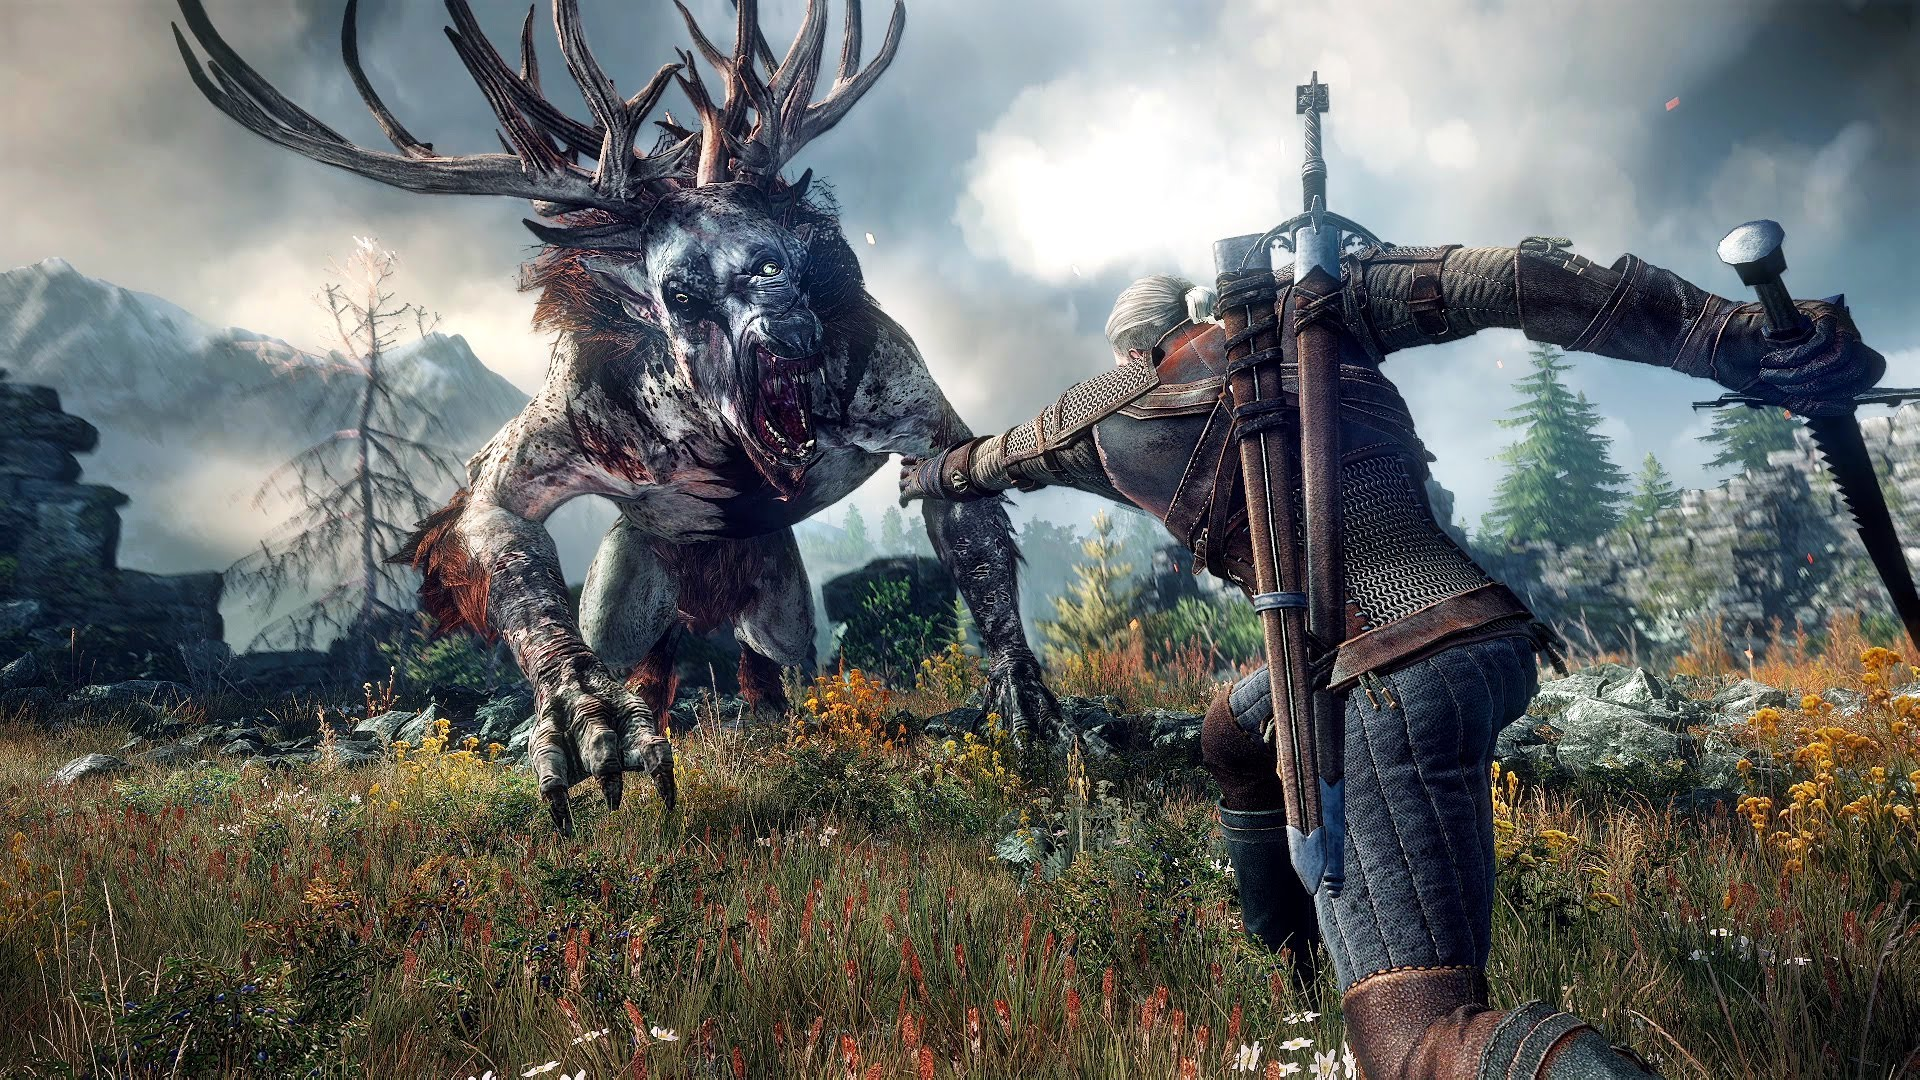
\includegraphics[scale=0.20]{img/whitcher.jpg}
	\caption{Contoh \textit{video game} dengan genre \textit{RPG}.}
	\label{fig:action_rpg}
\end{figure}
\vspace{1ex}

Pada dasarnya permainan dengan genre RPG (\textit{Role-Playing Game}) khususnya video game terbagi menjadi banyak kategori diantaranya adalah WRPG, JRPG, ARPG, TRPG, SRPG, dan MMORPG \citep{stenstrom2012}. Berikut adalah penjelasan selengkapnya:
\vspace{1ex}

\begin{subs}
	\subsection{WRPG}
	\label{sec:sub_sec2_wrpg}
	
	Deskripsi tentang genre WRPG (\textit{Western Role-Playing Game}) ini diambil dari \textit{Dungeons and Desktops: The History of Computer-Role-playing Games} oleh Barton. Namun seperti yang direpresenatasikan oleh Barton menggunakan istilah CRPG, sedangkan dalam penelitian ini istilah WRPG yang akan digunakan.
	\vspace{1ex}
	
	Pada WRPG pemain dapat bebas mengkostumisasi karakternya dengan leluasa seperti jenis kelamin, wajah dan lain sebagainya. Kemudian pemain juga dapat memilih kemampuannya yang direalisasikan dalam bentuk atribut atau stats dari karakter pemain tersebut \citep{barton2019}. Pada umumnya hal yang dipilih oleh pemain biasanya berupa suku atau fraksi seperti pada \textit{video game} berjudul \textit{The Elder Scroll V: Skyrim}, Bethesda (2011) seperti pada Gambar \ref{fig:skyrim}.
	\vspace{1ex}
	
	\begin{figure} [!h] \centering
		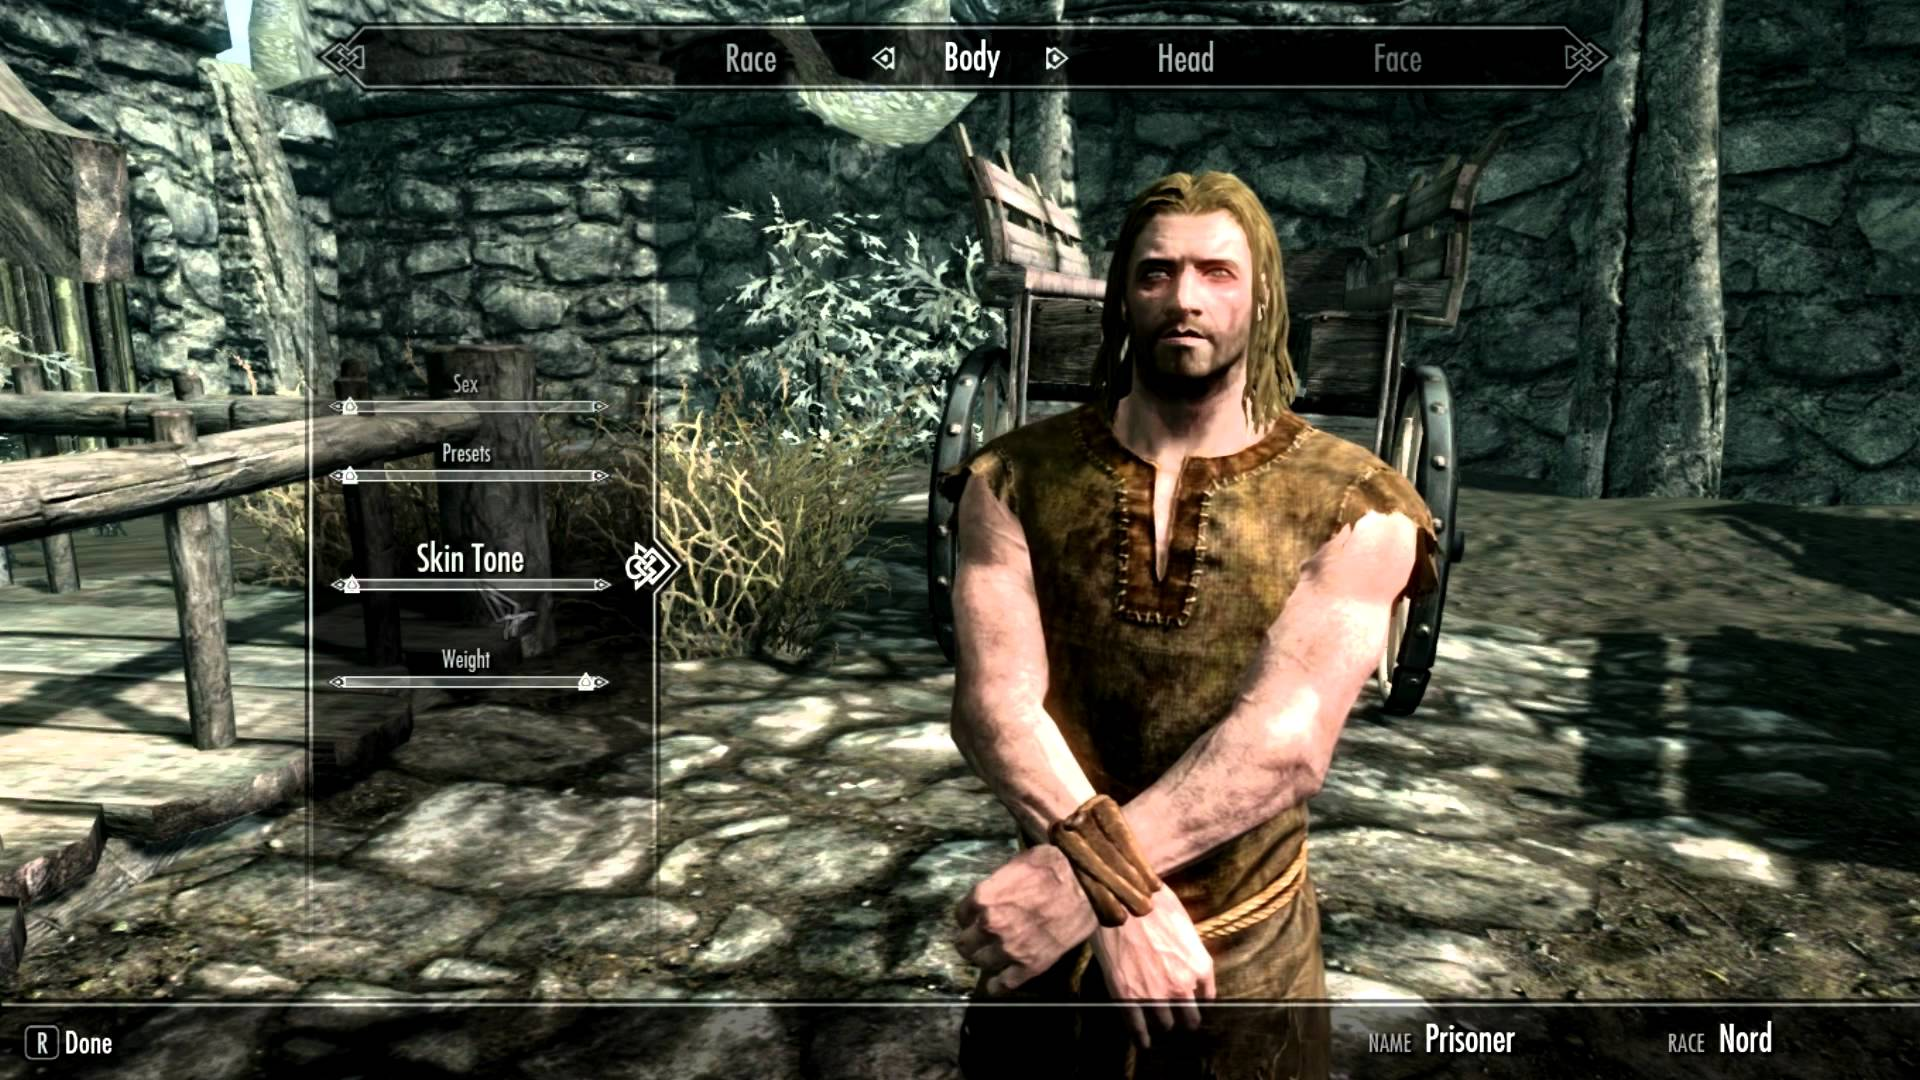
\includegraphics[scale=0.18]{img/skyrim.jpg}
		\caption{Contoh kustomisasi karakter pada WRPG.}
		\label{fig:skyrim}
	\end{figure}

	Sekumpulan musuh akan muncul sebelum permainan dimulai, dan pemain dapat menyiapkan perangkap atau membuat langkah kongkrit untuk mengalahkan sekumpulan  musuh tersebut. Sekumpulan musuh tersebut biasanya tersebar jumlahnya lebih banyak dari pemain. Atau mungkin pemain hanya berjumlah 1 dengan musuh yang berjumlah lebih dari itu, kemudian tugas dari pemain adalah mengalahkan sekumpulan musuh yang tersebar tersebut dengan melakukan pertarungan secara langsung atau \textit{real-time}, hal ini sangat identik dengan ARPG (akan dibahas pada poin selanjutnya).
	\vspace{1ex}
	
	Biasanya juga pada WRPG terapat banyak \textit{side quest} atau cerita sampingan yang berbeda dengan cerita utama. Hal ini memberikan pilihan jalan cerita untuk pemain dalam menyelesaikan permainan, selain itu karakter musuh dan juga boss dari musuh berbeda dengan misi atau cerita utama. Pada \textit{video game} berjudul \textit{The Witcher 3}, CD Pojekt (2015) memiliki banyak sekali cerita sampingan bahkan bisa dibilang cerita sampingan dari permainan tersebut tidak kalah bagusnya dengan cerita utama. Sekilas mengenai \textit{video game} berjudul \textit{The Witcher 3} dapat dilihat pada Gambar \ref{fig:action_rpg} pada bagian sebelumnya, yang mana dilakukan pertarungan secara \textit{real-time} melawan monster.
	\vspace{1ex}
	
	\subsection{JRPG}
	\label{sec:sub_sec2_jrpg}
	
	Pada mulanya permaian dengan genre JRPG (\textit{Japanese Role-Playing Game}) tidak begitu banyak mengandung kustomisasi karakter layaknya WRPG. Tetapi pada permainan RPG dengan genre ini berfokus pada beberapa karakter atau biasa disebut dengan istilah \textit{party member} yang dapat disusun oleh pemain. Sama seperti pada WRPG dimana pemain dapat mengkustomisasi kemampuan dari setiap \textit{party member} sesuai dengan peran masing-masing dengan tujuan untuk mengalahkan musuh. Dalam kostumisasi karakter pemain, biasanya diwujudkan dalam penambahan \textit{stats} dan penambahan jurus seperti pada \textit{video game} berjudul \textit{Shin Megami Tensei: Digital Devil Saga 1} dan \textit{2}, Atlus (2004, 2005) seperti yang ditunjukan pada Gambar \ref{fig:dds}.
	\vspace{1ex}
	
	\begin{figure} [!h] \centering
		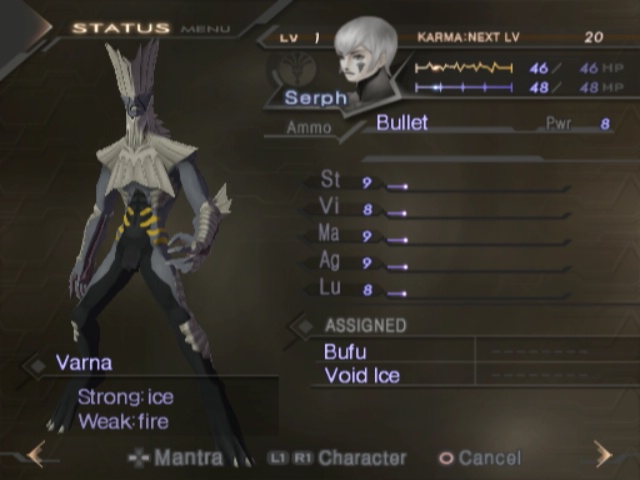
\includegraphics[scale=0.48]{img/dds.jpg}
		\caption{Contoh kustomisasi \textit{stats} pada JRPG.}
		\label{fig:dds}
	\end{figure}
	
	Pada mulanya pada permainan JRPG, pemain tidak mengetahui akan kedatangan musuh. Kedatangan musuh muncul secara tiba-tiba saat pemain melakukan pergerakan dalam peta permainan, hal ini biasa disebut denga istilah \textit{random encounter}. Contoh pada kondisi tersebut terdapat pada \textit{video game Shin Megami Tensei: Digital Devi Saga 1} dan \textit{2}. Jumlah musuh yang harus dilawan oleh \textit{party member} juga berjumlah lebih dari satu, sama-sama membentuk \textit{party member}.
	\vspace{1ex}
	
	Namun pada beberapa \textit{video game} JRPG, \textit{random encounter} juga direpresentasikan seperti monster atau bayangan yang mengejar representasi dari karakter pemain yang mewakili \textit{party member} dalam menjelajah dunia (eksplorasi). Setelah mereka bertabrakan maka terjadilah pertarungan antara \textit{party member} pemain dan musuh, seperti pada \textit{video game} berjudul \textit{Tales of Zestiria}, Bandai Namco (2015) dan juga \textit{Persona 4}, Atlus (2008).
	\vspace{1ex}
	
	Penataan strategi pada \textit{genre} JRPG bersifat sangat krusial, jika pada genre WRPG, ARPG dan SRPG pemain dapat mengganti perlalatan perangnya tetapi tidak pada genre JRPG. Pemain harus mempersiapkan segala seuatu dengan benar, apa saja yang dibutuhkan untuk mengalahkan musuh. Dalam mode pertarungan pada genre JRPG ada yang bersifat \textit{turn-based} seperti TRPG (akan dibahas pada poin selanjutnya) dan ada pula yang bersifat \textit{real-time} seperti WRPG.
	\vspace{1ex}
	
	Permainan berbasis \textit{turn-based} \citep{Panumate2015} adalah permainan yang memanfaatkan waktu secara diskrit, yang mana alur dari permainan khususnya pertarungan terbagi menjadi beberapa bagian yang disebut dengan giliran. Pada setiap giliran, pemain akan memiliki waktu yang terbatas atau tidak terbatas dalam berpikir dalam membuat keputusan setiap langkahnya. Kemudian sistem dari permainan akan memproses tindakan dari pemain. Kemudian permainan dilanjutkan oleh pemain berikutnya atau musuh yang berupa AI akan melakukan giliran selanjutnya seperti pada Gambar \ref{fig:turn_based}.
	\vspace{2ex}
	
	\begin{figure} [!h] \centering
		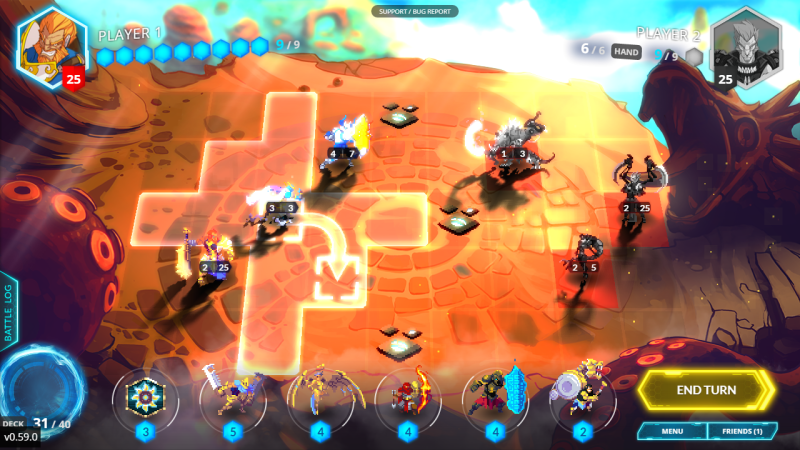
\includegraphics[scale=0.42]{img/duelyst.png}
		\caption{Contoh permainan digital dengan genre \textit{turn-based}.}
		\label{fig:turn_based}
	\end{figure}

	Pada Gambar \ref{fig:persona4} adalah mode pertarungan JRPG secara \textit{turn-based} yang dicontohkan oleh \textit{Persona 4}, Atlus (2008). Di mana para karakter yang dimainkan oleh pemain harus melakukan serangan secara bergatian yang kemudian baru dilanjutkan dengan serangan dari musuh.
	\vspace{1ex}
	
	\begin{figure} [!h] \centering
		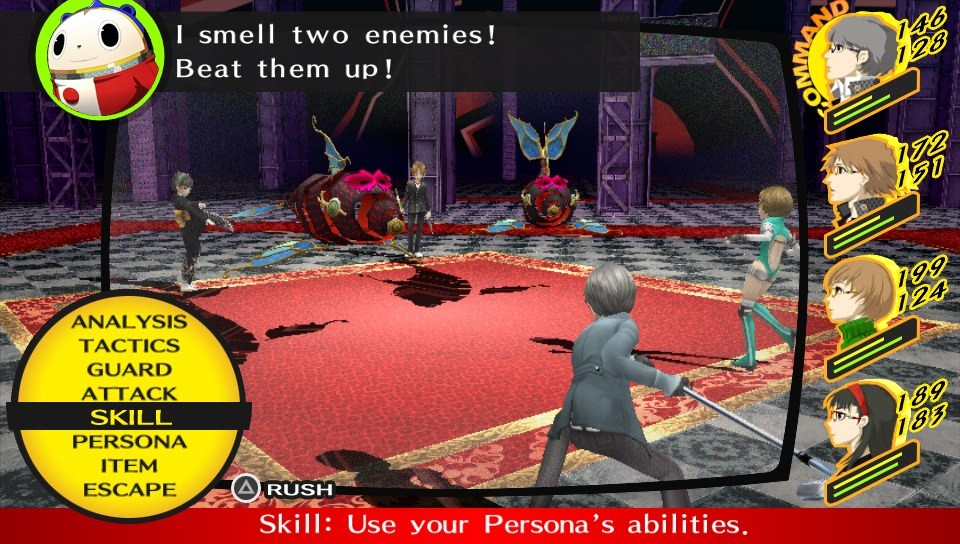
\includegraphics[scale=0.35]{img/persona4.jpg}
		\caption{Mode pertarungan \textit{turn-based} pada JRPG.}
		\label{fig:persona4}
	\end{figure}
	
	Pada Gambar \ref{fig:tales} adalah mode pertarungan JRPG secara \textit{real-time} yang dicontohkan oleh \textit{Tales of Zestiria}, Bandai Namco (2015). Di mana pemain menentukan formasi dalam party member, siapa saja karakter yang akan bertarung dan \textit{skill} apa saja yang dibutuhkan untuk mengalahkan musuh. Saat berlangsungnya pertarungan hanya satu karakter yang dapat dijalankan oleh pemain, tetapi pemain diberikan kelebihan untuk berganti karakter dalam pertarungan atau \textit{switch}.
	\vspace{1ex}
	
	\begin{figure} [!h] \centering
		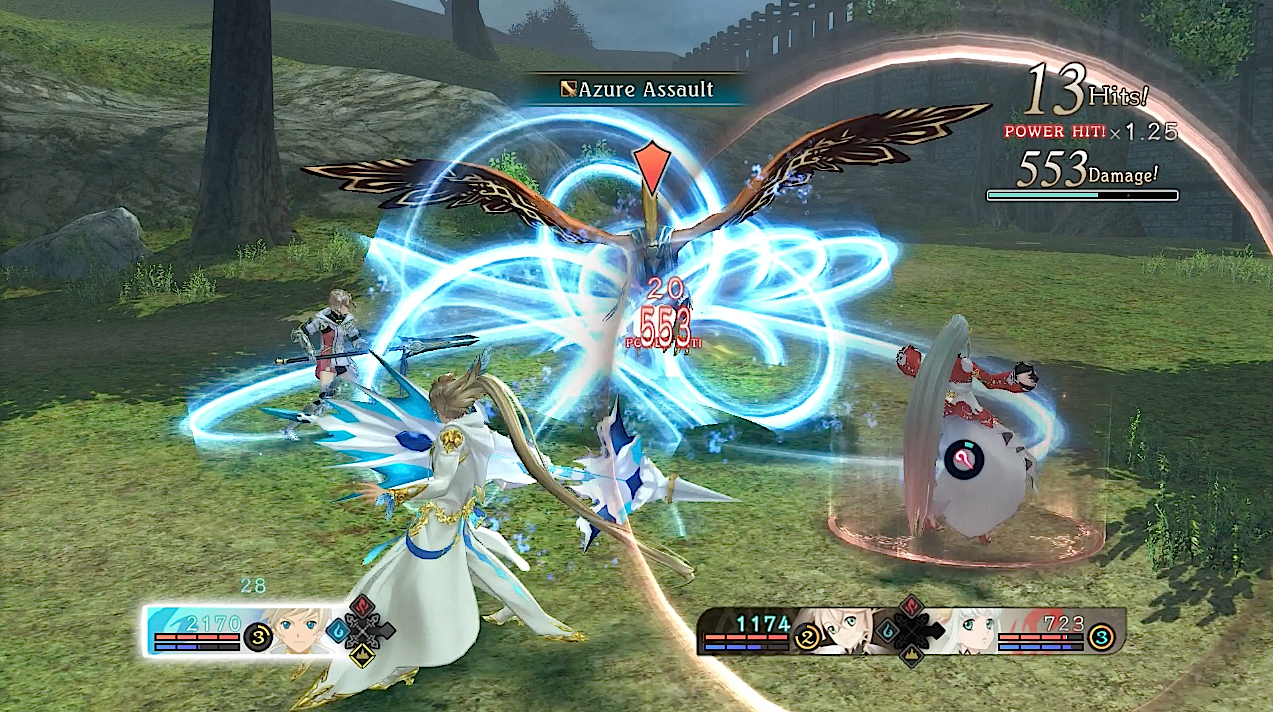
\includegraphics[scale=0.26]{img/tales.png}
		\caption{Mode pertarungan \textit{real-time} pada JRPG.}
		\label{fig:tales}
	\end{figure}
	
	Sama seperti dengan WRPG pada JRPG juga memiliki \textit{side-quest} tetapi biasanya hanya berupa permainan kecil saja, yang bersifat memainkan permainan lain diluar pertarungan antar \textit{party member}. Selain itu juga terdapat \textit{secret boss} yang bersifat sangat kuat dan sulit dikalahkan. Kemudian adanya \textit{new game+}, yang memungkinkan pemain untuk tetap memainkan karakter dengan kemampuan yang sama seperti permainan sebelumnya dan adanya penambahan konten untuk dimainkan (biasanya \textit{boss} yang lebih banyak).
	\vspace{1ex}
	
	\subsection{ARPG}
	\label{sec:sub_sec2_arpg}
	
	Biasanya genre ini disebut juga dengan ``\textit{Hack and Slash}" atau ``\textit{Dungeon crawl RPG's}" \citep{moore2016}. Kenapa sampai diberi sebutan ``\textit{Hack and Slash}", hal ini mengacu dari kesederhanaan dari beberapa permainan ARPG. Pada permainan RPG jenis ini (khususnya \textit{video game}) berfokus pada aksi atau ketangkasan seperti memukul, menghindar, mengeluarkan jurus dan lain sebagainya dibandingkan dengan pengaturan strategi atau penyusunan \textit{stats}. Jika melihat cara bertarung pada permainan jenis ini, maka akan sangat mirip sekali dengan WRPG yang mana pemain fokus dalam bertarung dan berekplorasi. Contoh genre ini adalah \textit{Diablo}, Blizzard (1997) dan \textit{Final Fantasy 12}, Square Enix (2006).
	\vspace{1ex}
	
	\subsection{TRPG}
	\label{sec:sub_sec2_trpg}
	
	Pada RPG jenis ini tidak memiliki dunia atau maps yang digunakan untuk bereksploarsi sama sekali. Jadi pemain tidak perlu berkeliling sama sekali, sedangakan untuk sisi cerita pemain hanya melihat interaksi antar karakter atau interaksi antara karakter pemain dengan karakter musuh yang membentuk sebuah cerita.
	\vspace{1ex}
	
	Jumlah karakter yang dimainkan oleh pemain biasanya berjumlah sangat banyak dan terpapar dalam sebuah panel isometrik atau kotak, dan disanalah dilakukannya pertarungan antara karakter-karakter dari pemain melawan musuh-musuh. Pada RPG genre ini sangat berbanding terbalik dengan ARPG, yang mana pada TRPG sama sekali tidak membutuhkan aksi. Dalam artian tidak diperlukannya ketangkasan dalam melakukan serangan atau dalam menghindari serangan musuh, yang sangat diperlukan adalah 100\% perencanaan dan strategi. Pertarungan benar-benar dilakukan secara bergantian antara pemain dan musuh dalam melakukan serangan \citep{moore2016}. Contoh dari permainan dengan genre ini adalah \textit{Advance Wars}, Nintendo (2001). Penjelasan dari \textit{turn-based} atau bergantian sudah dijelaskan juga pada Sub-Bab \ref{sec:sub_sec2_jrpg} dan juga dicontohkan dengan \textit{video game} yang berjudul \textit{Duelyst}, Counterplay Games (2016).
	\vspace{1ex}
	
	Hampir sebagian besar permainan dengan genre ini berasal dari pengembang \textit{video game} asal jepang selayaknya JRPG. Terdapat juga versi lain TRPG, dengan adanya penambahan atribut \textit{speed} atau kecepatan yang menentukan karakter mana yang akan melakukan aksi terlebih dahulu. Contoh dari permainan tersebut terdapat pada \textit{Final Fantasy Tactics}, Square (1997).
	\vspace{1ex}
	
	\subsection{SRPG}
	\label{sec:sub_sec2_srpg}
	
	Genre RPG ini adalah termasuk yang paling modern, pada penelitian ini \textit{shooter} RPG dipersingkat menjadi SRPG. Biasanya istilah SRPG rancu dengan TRPG, yang mana S tersebut diartikan menjadi \textit{strategy}. SRPG sangat mirip sekali dengan ARPG hanya saja senjata utama dari permain ini menggunakan senapan atau panahan. Mengingat RPG jenis ini adalah \textit{shooter}, bukan berarti prespektif dari permainan ini adalah FPS (\textit{First Person Shooter}). Bisa jadi juga prespektifnya adalah \textit{third person} atau bahkan pemain bisa memilih mode yang mereka inginkan seperti pada \textit{video game} berjudul \textit{Fallout 4}, Bethesda (2015).
	\vspace{1ex}
	
	\subsection{MMORPG}
	\label{sec:sub_sec2_mmorpg}
	
	Kebanyakan \textit{gameplay} dari MMORPG (\textit{Masive Multiplayer Online Role-Playing Game}) terbagi menjadi dua jenis. Pertama adalah \textit{gameplay} yang mengedepankan kenaikan level dan selanjutnya adalah \textit{gameplay} yang mengedepankan penguatan karakter berdasarkan item yang dimiliki dalam memperankan perannya. Genre ini sangat mirip dengan WRPG dan JRPG, namun dijalankan secara \textit{online} atau daring yang mempertemukan banyak pemain.
	\vspace{1ex}
	
	Pada MMORPG yang mirip dengan WRPG, terdapat pada bagian pembuatan karakter, dan pertempuran secara \textit{real-time} meskipun tidak benar-benar \textit{real-time}. Selain itu, pada MMORPG yang memiliki pola permainan khas JRPG \citep{moore2016}. Di contohkan dengan adanya \textit{boss} dan banyak musuh dengan susunan dan kemampuan yang sudah terpola. Pertempuran sering kali mengharuskan para pemain untuk bergerak dan menghindari kemampuan musuh, kemudian melakukan serangan disaat yang tepat.
	
\end{subs}